\documentclass[a4paper,12pt]{mwart}

\usepackage[english,polish]{babel}
\usepackage[utf8]{inputenc}
\usepackage[T1]{fontenc}
\usepackage{indentfirst}
\usepackage{polski}
\frenchspacing

\usepackage{dirtree}
\usepackage{enumerate}
\usepackage{csquotes}
\usepackage{graphicx}
\usepackage{float}
\usepackage{makecell}
\usepackage{siunitx}
\sisetup{output-decimal-marker = {,}}
\usepackage{icomma}
\let\lll\undefined
\usepackage{amsmath, amssymb, amsfonts}
\usepackage{mathtools}
\usepackage{setspace}
\usepackage{import}
\usepackage[all,defaultlines=2]{nowidow}

\usepackage[%
style=numeric,
sorting=none,
language=autobib,
autolang=other,
backend=biber,
]{biblatex}

\usepackage{listings}
\usepackage{color}

\floatstyle{plaintop}
\ifcsname{chapter}\endcsname%
    \newfloat{program}{!tbh}{lop}[chapter]
\else%
    \newfloat{program}{!tbh}{lop}
\fi
\floatname{program}{Kod źr.}

\definecolor{mygreen}{rgb}{0,0.6,0}
\definecolor{mygray}{rgb}{0.5,0.5,0.5}
\definecolor{mymauve}{rgb}{0.58,0,0.82}

\lstset{ %
  backgroundcolor=\color{white},     % choose the background color
  basicstyle=\ttfamily\footnotesize, % size of fonts used for the code
  breaklines, breakatwhitespace,     % automatic line breaking only at whitespace
  commentstyle=\color{mygreen},      % comment style
  numbers=left,
  showstringspaces=false,
  numberstyle=\tiny,
  frame=l,
  language=Python,
  escapeinside={\%*}{*)},            % if you want to add LaTeX within your code
  keywordstyle=\color{blue},         % keyword style
  stringstyle=\color{mymauve}        % string literal style
}

\lstset{%
  literate={ą}{{\k{a}}}1
  {ć}{{\'c}}1
  {ę}{{\k{e}}}1
  {ó}{{\'o}}1
  {ń}{{\'n}}1
  {ł}{{\l{}}}1
  {ś}{{\'s}}1
  {ź}{{\'z}}1
  {ż}{{\.z}}1
  {Ą}{{\k{A}}}1
  {Ć}{{\'C}}1
  {Ę}{{\k{E}}}1
  {Ó}{{\'O}}1
  {Ń}{{\'N}}1
  {Ł}{{\L{}}}1
  {Ś}{{\'S}}1
  {Ź}{{\'Z}}1
  {Ż}{{\.Z}}1
}

\AtBeginDocument{
  \renewcommand{\tablename}{Tab.}
  \renewcommand{\figurename}{Rys.}
}

\usepackage{placeins}

\let\Oldsection\section
\renewcommand{\section}{\FloatBarrier\Oldsection}

\let\Oldsubsection\subsection
\renewcommand{\subsection}{\FloatBarrier\Oldsubsection}

\let\Oldsubsubsection\subsubsection
\renewcommand{\subsubsection}{\FloatBarrier\Oldsubsubsection}


\usepackage{csquotes}
\DeclareQuoteAlias{croatian}{polish}

\addbibresource{bibliografia.bib}

\begin{document}

\onehalfspacing
\begin{flushleft}

  \textbf{Szymon \MakeUppercase{Mikulicz}} \\
  \textbf{Marcel \MakeUppercase{Piszak}} \\
  \vspace*{12pt}

  \MakeUppercase{\textbf{Wibroakustyczna stacja pomiarowa oparta o mikrokomputer Raspberry Pi}} \\
  \vspace*{6pt}
  \MakeUppercase{\textbf{Vibroacoustic measuring station based on Raspberry Pi microcomputer}} \\
  \vspace*{12pt}

  AGH Akademia Górniczo-Hutnicza \\
  Wydział Inżynierii Mechanicznej i Robotyki \\
  Katedra Mechaniki i Wibroakustyki \\
  \vspace*{6pt}

  czilukim@o2.pl \\
  marcel.piszak@wp.pl \\

\end{flushleft}

\noindent
\textbf{Streszczenie} \\
Treść streszczenia
\vspace*{24pt}

\noindent
\textbf{Abstrakt} \\
Współczesne rozwiązania dedykowane do pomiarów drgań budynków proponowane przez
popularnych producentów sprzętu pomiarowego charakteryzują się dużym stopniem
skomplikowania. Celem niniejszego projektu było zbudowanie prostego i
przystępnego cenowo systemu pozwalającego na pomiar i analizę drgań budynków
zgodną z normą PN-B 02170:2016-12. Postanowiono stworzyć system pomiarowy
oparty na platformie Raspberry Pi® oraz wykorzystujący akcelerometry typu MEMS
w celu minimalizacji kosztów i rozmiarów stacji. Oprogramowanie kontrolujące
akwizycję oraz analizę danych napisano przy użyciu języka Python i odpowiednich
bibliotek. Skonstruowanie oraz uruchomienie zaprogramowanego układu ma
bezpośrednio przyczynić się do realizacji większego projektu obejmującego
połączenie takich jednostek analizujący drgania na większym obszarze.
\vspace*{24pt}


\section{Wstęp}

Pomiary drgań są ważnym elementem oceny wibroakustycznej w technice. Jednym
z wielu pól na których można je stosować jest badanie wpływu wibracji
podłoża na budynki. Źródła drgań oddziałujące na obiekty budowlane są
zróżnicowane, ale najczęściej pochodzą od wszelkich środków transportu
eksploatowanych w bezpośredniej bliskości zabudowy. W miastach wzmożona
komunikacja samochodowa, ruch tramwajowy, a nawet metro potrafią powodować
występowanie drgań o dużych amplitudach przyspieszeń. Z kolei konstrukcje
budynków poddawane długotrwałej ekspozycji na drgania mogą ulegać
uszkodzeniom, a w skrajnych przypadkach zniszczeniu. Dodatkowo na terenach
miejskich często można spotkać budynki wymagające dużego ograniczenia wpływu
drgań za względu na pełnione funkcje. Różnego rodzaju laboratoria, szpitale
czy przemysł precyzyjny nie dopuszczają występowania drgań o amplitudach
uniemożliwiających pełnienie danej funkcji przez mieszczący je budynek.

Istnieją różne metody pomiaru oraz analizy drgań oddziałujących na budynki
jednak pewne dokumenty normatywne pozwalają na określenie wpływu drgań oraz
weryfikację pomiarową i późniejsze porównania, czy też odniesienie wyników
do wartości dopuszczalnych. Norma PN-B 02170:2016-12 pod tytułem ,,Ocena
szkodliwości drgań przekazywanych przez podłoże na budynki'' \cite{norma}
zawiera przede wszystkim metodykę oceny wpływu drgań, ale można w niej
znaleźć również unormowane zasady wykonywania pomiarów.

\section{Przegląd dostępnych rozwiązań}

Na przestrzeni ostatnich lat popularne stało się wykorzystanie platform
komputerowych wspierających naukę programowania takich jak Arduino czy Raspberry
Pi do tworzenia wszelkiego rodzaju jednostek pomiarowych. Takie aplikacje
znajdują również zastosowania w pomiarach wibroakustycznych. Platforma Raspberry
Pi, ponieważ w zasadzie jest samodzielnym komputerem z systemem operacyjnym
opartym na jądrze Linux, daje duże możliwości tworzenia samodzielnych systemów
pomiarowych. Do tej pory dominującym podejściem pomiarowym drgań oraz hałasu
jest wykorzystanie analogowego przetwornika będącego osobnym elementem toru
pomiarowego. Sygnał analogowy jest przesyłany z reguły do karty pomiarowej, a
następnie, pod postacią cyfrową, trafia do komputera który jest odpowiedzialny
za jego analizę. W wielu przypadkach duża dokładność pomiaru wymusza
zastosowanie profesjonalnych, wyspecjalizowanych przetworników, ale niekiedy
zdarza się, że sygnał pomiarowy nie wymaga bardzo dużej rozdzielczości lub
częstotliwości próbkowania. Podejmowano już pracę nad stworzeniem systemów
analizy drgań opartym na platformie Raspberry Pi. Przykładem może być praca pod
tytułem ,,Development of a system for monitoring vibration accelerations based
on the Raspberry Pi microcomputer and the ADXL345 accelerometer''~\cite{art1}.
Autorzy publikacji skupili się na opracowaniu systemu monitorowania i analizy
drgań na podstawie widma, tak aby łatwo dało się go dostosować do środowiska
działania. 

\section{Założenia projektowe}

Głównym założeniem projektu była prostota konstrukcji, dostępność elementów i
ich zgodność z wymogami pomiarów określonych w normie \cite{norma}. Charakter
sygnału drgań mierzonego na potrzeby normy określają następujące parametry:
\begin{itemize}
  \item Pasmo częstotliwości od \SI{0,5}{\hertz} do \SI{100}{\hertz}
  \item Amplituda prędkości drgań od \SI{e-4}{\metre\per\second} do \SI{1}{\metre\per\second}
  \item Amplituda przyspieszenia drgań od \SI{e-3}{\metre\per\square\second} do \SI{10}{\metre\per\square\second}
\end{itemize}
Norma wskazuje również na posiadanie możliwości zapisu w pamięci urządzenia
zarejestrowanych wibrogramów. Analiza powinna być prowadzona w pasmach
tercjowych. W procesie przetwarzania i analizy sygnału wykorzystano wyłącznie
biblioteki na licencji wolnego oprogramowania, a cały kod napisany podczas jego
realizacji umieszczono na platformie GitHub.

\section{Opis realizacji projektu}

Stacja pomiarowa będąca przedmiotem niniejszego projektu została oparta o
platformę Raspberry Pi 3 model B. Jako czujnik drgań wybrano moduł
akcelerometru MEMS MMA8451 firmy Adafruit~\cite{mma8451}. Jest on niewielkich
rozmiarów, pozwala na pomiar przyspieszenia drgań w trzech osiach jednocześnie.
Posiada wbudowany, 14-bitowy przetwornik analogowo-cyfrowy oraz ma możliwość
komunikacji z mikroprocesorem za pomocą interfejsu I\textsuperscript{2}C. Warto
także zaznaczyć, że akcelerometr ten pozwala na wybór jednego z trzech
dostępnych zakresów pomiarowych: $\pm$\SI{2}{\g}, $\pm$\SI{4}{\g} oraz
$\pm$\SI{8}{\g}.  Częstotliwość próbkowania także może być zmieniana przez
użytkownika, a jej największa wartość to \SI{800}{\hertz}. Akcelerometr posiada
również wiele wbudowanych funkcji, między innymi filtr górnoprzepustowy.

Jako system operacyjny dla mikrokomputera wybrano Rasbian -- przygotowaną
specjalnie dla Raspberry Pi dystrybucję Linuxa. Wybrano wersję Lite, jedynie z
obsługą z poziomu terminala. Komunikacja z komputerem pozwalająca na
oprogramowanie oraz obsługę stacji odbywała się przez protokół SSH.
Mikrokomputer posada zarówno złącze Ethernet jak i moduł Wi-Fi, co umożliwia
podłączenie go do sieci LAN. Użyto kart pamięci o pojemności 16 GB aby możliwe
było chwilowe zapisywanie pełnych przebiegów sygnałów drganiowych.

\begin{figure}[!tbh]
  \centering
  \import{vecgraphics/}{schemat.pdf_tex}
  \caption{Schemat stworzonego systemu pomiarowego}
  \label{fig:schemat}
\end{figure}

Użyty do komunikacji z mikroprocesorem protokół I\textsuperscript{2}C jest
protokołem szeregowym oraz synchronicznym. Jego warstwa fizyczna składa się z
linii danych (SDA) oraz linii zegarowej (SCL). I\textsuperscript{2}C korzysta z
logiki odwróconej, a jego warstwa łącza danych oparta jest o system bajtowy. Po
przesłaniu 8-bitowej ramki danych następuje wysłanie bitu potwierdzającego
odbiór. Aby transmisja była możliwa konieczne jest zastosowanie rezystorów
podciągających do linii zasilania. Zostały one uwzględnione przez producenta
modułu akcelerometru i są umieszczone na płytce drukowanej. Dodatkowe dwie
linie to zasilanie modułu, którego napięcie, dzięki wewnętrznemu regulatorowi
napięcia, może zawierać się w przedziale od $+$\SI{3.3}{\volt} do
$+$\SI{5}{\volt} (VIN) oraz potencjał masy (GND).  Ostatnią linię stanowi linia
sygnału przerwania (I1), której działanie zostanie opisane później.

\begin{figure}[!tbh]
  \centering
  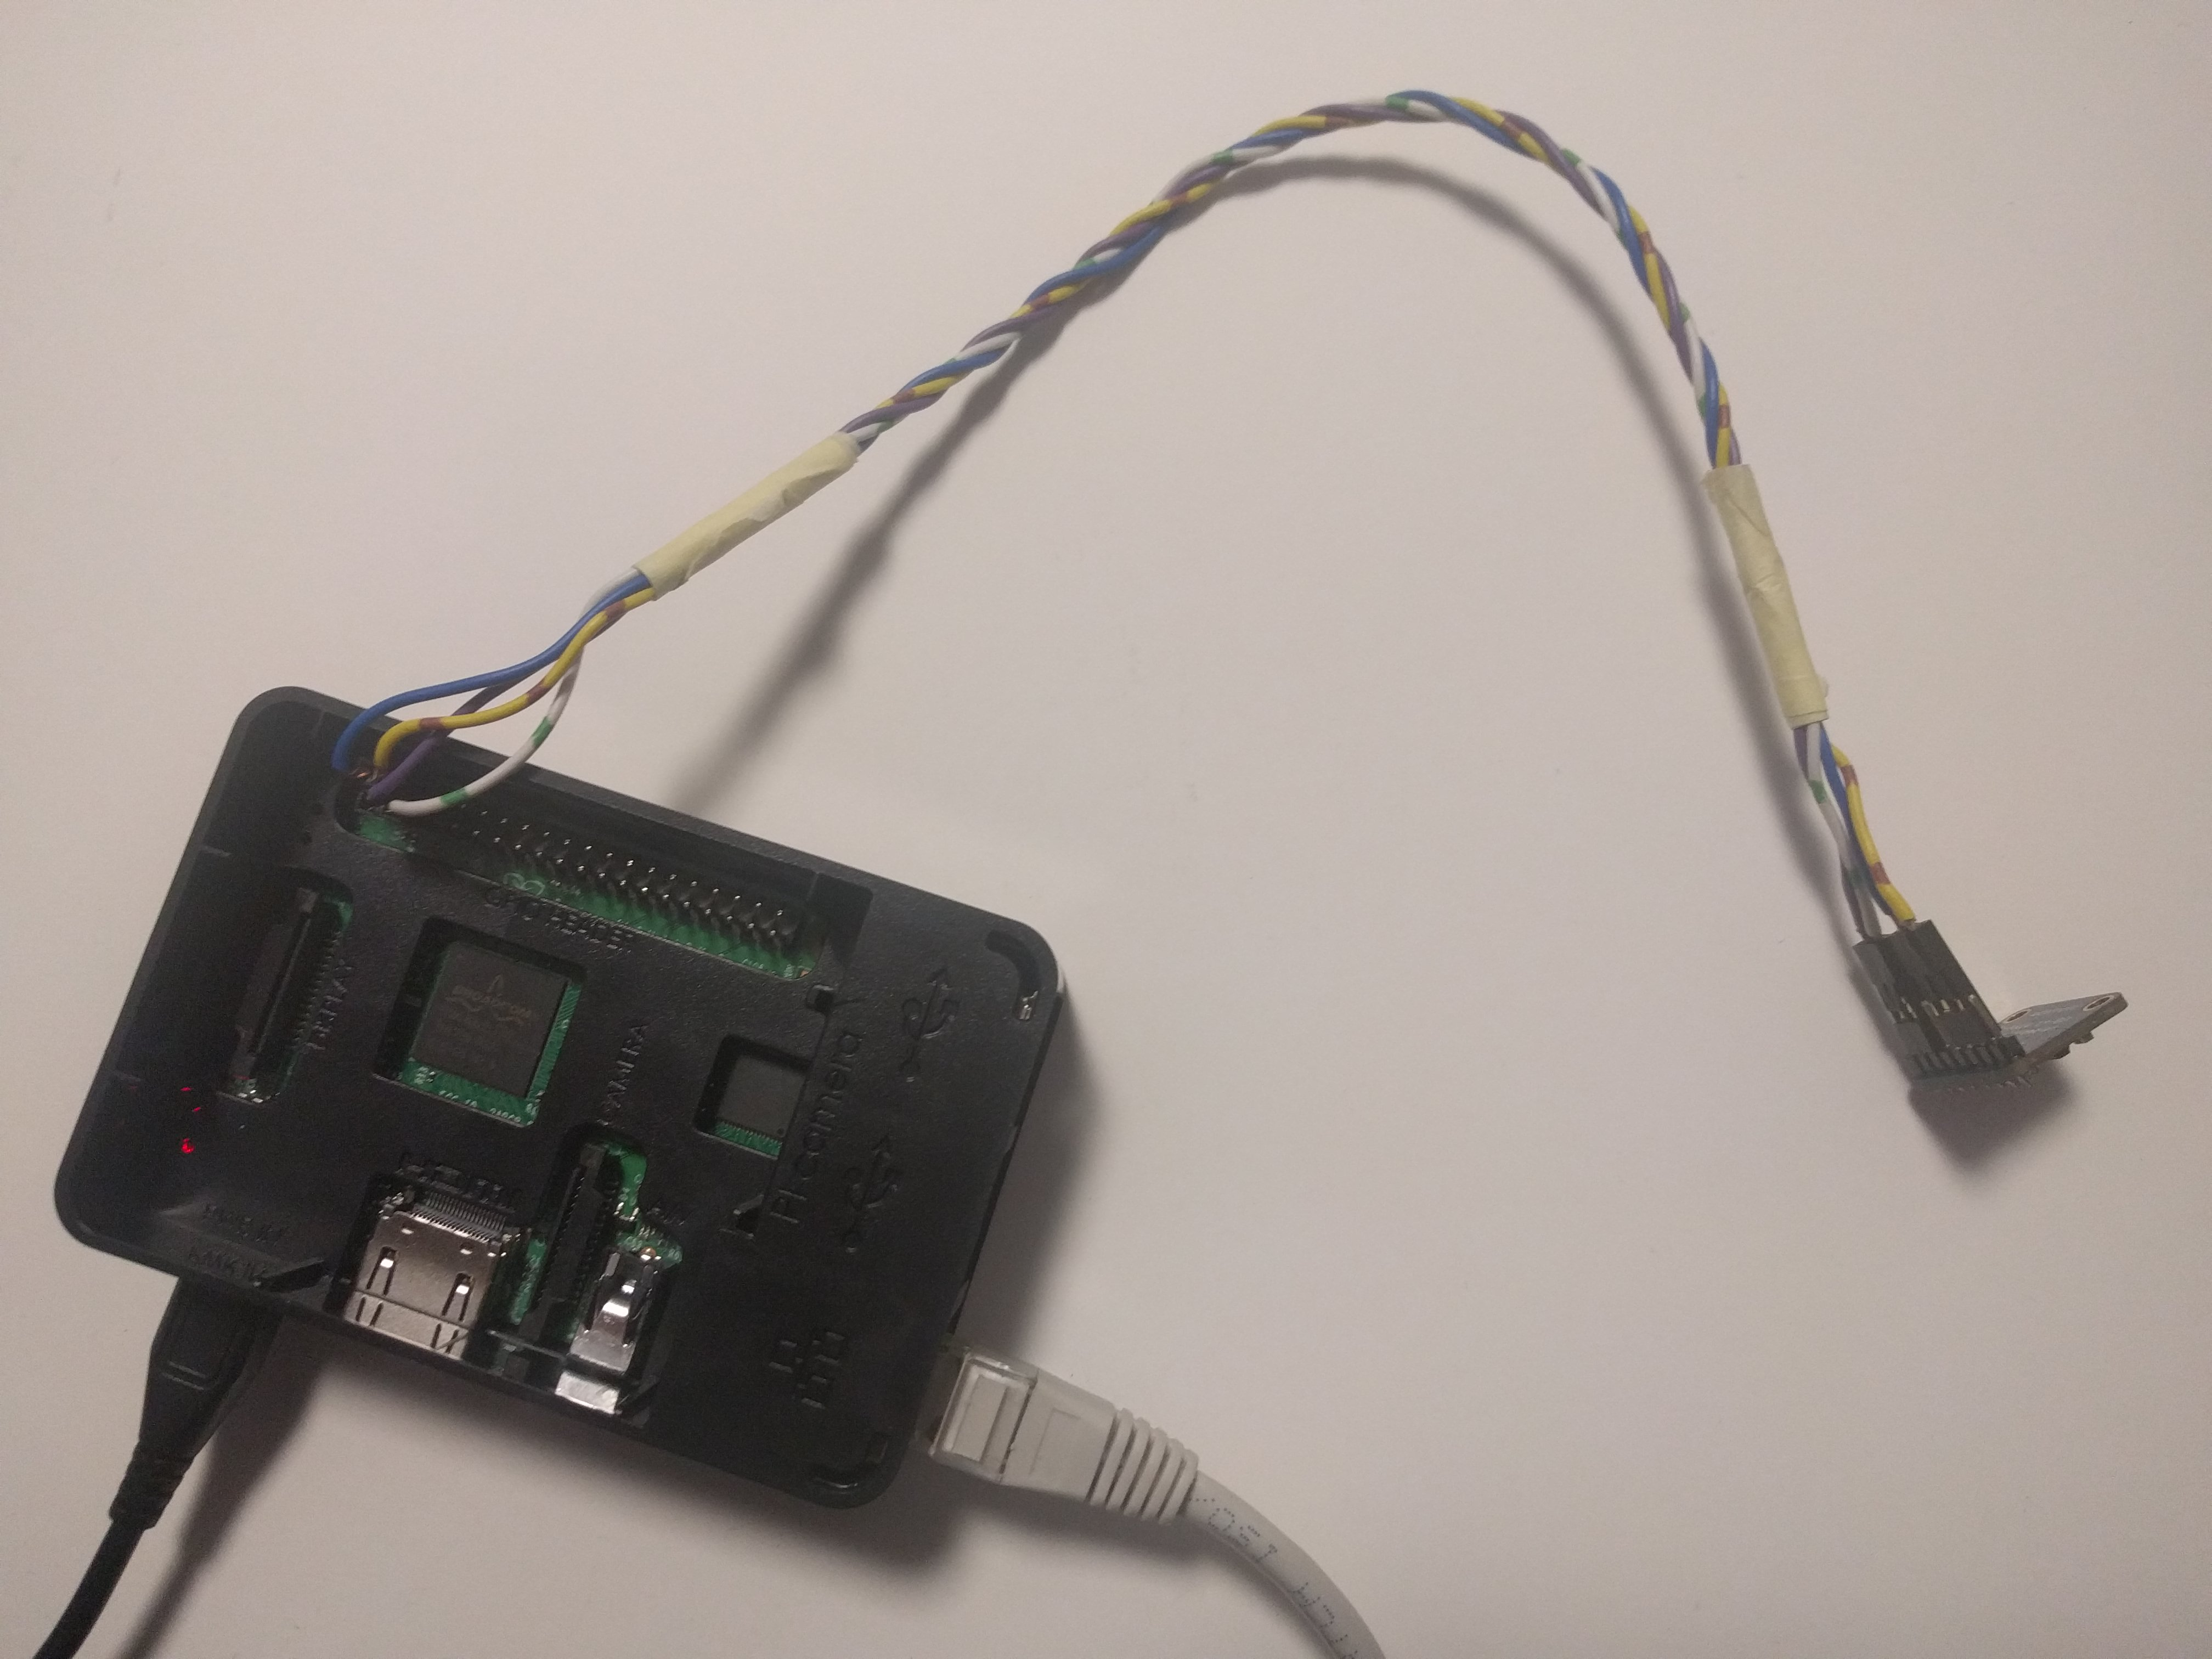
\includegraphics[width=\textwidth]{bitgraphics/pi.png}
  \caption{Wibroakustyczna stacja pomiarowa}
  \label{fig:foto}
\end{figure}

Od strony mikrokomputera Raspberry Pi obsługę wyżej wymienionych linii zapewnia
panel GPIO (General Purpose Input Output). Znajdują się w nim piny zasilające,
uziemienia, piny dedykowanych do konkretnych protokołów komunikacji, w tym
I\textsuperscript{2}C, i piny których przeznaczenie nie jest ustalone.  Na
poziomie oprogramowania do obsługi komunikacji przez wybrany protokół pomocny
jest pakiet narzędzi {\fontfamily{\ttdefault}\selectfont i2c-tools}, który
między innymi pozwala odczytać adres urządzeń podłączonych do magistrali.

Główną częścią projektu było napisanie biblioteki do obsługi używanego
akcelerometru, oraz kodu który ją wykorzystuje w celu nieprzerwanej akwizycji i
zapisu danych pomiarowych. Dokładne działanie urządzenia zostało opisane w
dokumentacji \cite{mma8451}. Komunikacja z urządzeniem, przez protokół
I\textsuperscript{2}C, polegała na zapisie i odczycie danych z rejestrów.
Pierwszym krokiem było stworzenie części biblioteki która w wygodny sposób
pozwoli ustawiać flagi (kombinacje bitów w rejestrach, które sygnalizują
urządzeniu pożądaną konfigurację) i odczytywać dane z tych rejestrów. W tym
celu stworzono klasy \lstinline|Flag| i \lstinline|Register|, które
przechowują liczby odpowiadające odpowiednio kombinacji bitów flagi i
adresowi rejestru (Kod źr. \ref{code:reg}).

\begin{program}
  \caption{Definicja rejestru \lstinline|STATUS| i jego flag}
  \begin{lstlisting}
    import mma8451.register.addr as REG
    from mma8451.register.classes import Flag

    class STATUS(Flag):
      _addr           = REG.STATUS
      ZYXOW           = 0x80
      ZOW             = 0x40
      YOW             = 0x20
      XOW             = 0x10
      ZYXDR           = 0x08
      ZDR             = 0x04
      YDR             = 0x02
      XDR             = 0x01
  \end{lstlisting}
  \label{code:reg}
\end{program}

Następnie stworzono klasę \lstinline|IIC|, która, posiada metody pozwalające na
zapis wartości do rejestrów, jak i odczyt wartości przy wykorzystaniu uprzednio
stworzonych typów. Szczególnie ważne było stworzenie metody pozyskiwania
wartości w trybie \emph{burst}, który pozwala na odczyt wielu wartości naraz
jednym ciągiem danych. Wykorzystuje ona bibliotekę \emph{pigpio}.

\begin{program}
  \caption{Wykorzystanie klasy IIC do poboru danych}
  \begin{lstlisting}
    from mma8451.register import register as REG
    from mma8451.iic import IIC
    import pigpio

    # Inicjalizacja połączenia z procesem pigpio
    pi = pigpio.pi()
    # Stwórz obiekt klasy, gdzie 1 do magistrala a 0x1D adres
    iic = IIC(pi, 1, 0x1D)
    # Uśpij urządzenie
    iic.unset_flag(REG.CTRL_REG1.ACTIVE)
    # Włącz tryb 14-to bitowy
    iic.unset_flag(REG.CTRL_REG1.F_READ)
    # Włacz urządzenie do trybu aktywnego
    iic.set_flag(REG.CTRL_REG1.ACTIVE)
    # Pobierz dane ze wszystkich trzech osi
    dane = iic.block_read(REG.OUT_X_MSB, 6)
  \end{lstlisting}
  \label{code:iic}
\end{program}

Po napisaniu tych elementów biblioteki zajęto się jej główną częścią, służącą
do inicjalizacji urządzenia, obsługi przerwań, ustawienia pożądanych parametrów
i przygotowania wątków i procesów ciągłej akwizycji i zapisu danych. W procesie
inicializacji ustawiane są flagi włączające tryb niskoszumowy urządzenia oraz
najmniej energooszczędny, natomiast najbardziej dokładny tryb próbkowania.
Ustawienia zakresu dynamicznego oraz częstotliwości próbkowania pozostawione są
na swoich domyślnych wartościach, odpowiednio $\pm\SI{2}{\g}$ oraz
\SI{800}{\hertz}. Pozwala to zapewnić maksymalną dokładność uzyskanych z
urządzenia danych.

Kolejno ustawiane są flagi które aktywują wbudowaną kolejkę FIFO (First In
First Out) urządzenia. Aby nie stracić żadnych próbek z powodu tymczasowego
spowolnienia wykonywania programu oraz by nie zajmować całego czasu procesora
poprzez ciągłe sprawdzanie rejestrów w oczekiwaniu na nowe próbki, jest
wykorzystana ta kolejka, która może przechowywać aż do trzydziestu dwóch
czternasto-bitowych próbek z trzech osi. Kolejka jest ustawiana tak, by w
momencie wykroczenia liczby próbek w kolejce ponad dwadzieścia następowało
przerwanie, wysyłane w postaci zmiany stanu na pinie \emph{I1} do GPIO.
W programie ustawiona jest by w momencie wykrycia tej zmiany została wykonana
funkcja, która informuje wątek akwizycji o dostępności nowych danych.

Po inicjalizacji ustawień uruchamiany jest wątek akwizycji danych oraz proces,
który się zajmuje ich zapisywaniem. Wątek akwizycji czeka na informację o
dostępności nowych danych po czym odczytuje wszystkie próbki z kolejki
wykorzystując do tego wspomniany wcześniej tryb \emph{burst}, a następnie
zebrane wartości przekazuje do kolejki. Na dane w kolejce czeka proces
zapisujący, który po zebraniu odpowiedniej ilości próbek, która w tym momencie
odpowiada pięciu minutom, przeprowadza zamianę uzyskanych wartości z kodu
uzupełnień do dwóch na liczbę całkowitą ze znakiem, po czym uzyskaną macierz
zawierającą dane ze wszystkich osi zapisuje do plik HDF5 w grupach
odpowiadających dacie i godzinie zapisu. Wybrano format HDF5 z powodu na jego
uniwersalność oraz wygodę wewnętrznej struktury (Rys. \ref{fig:struc}).

\begin{figure}[!tbh]%
  \centering%
  \begin{minipage}{0.3\textwidth}%
    \dirtree{%
      .1 <rok>/.
      .2 <miesiąc>/.
      .3 <dzień>/.
      .4 <godzina>/.
      .5 <minuta>.
      .5 \dots.
      .4 \dots.
      .3 \dots.
      .2 \dots.
    }%
  \end{minipage}%
  \caption{Struktura grup w pliku z danymi}%
  \label{fig:struc}%
\end{figure}%

% opis kodu

Stacja pomiarowa jest zdolna do zapisania w swojej pamięci wewnętrznej około
miesiąca wibrogramu. Ponieważ norma wymaga analizy tercjowej drgań, uwzględniono
filtrację sygnału w pasmach od \SI{0,5}{\hertz} do \SI{100}{\hertz}.

\begin{figure}[!tbh]
  \centering
  \includegraphics[width=0.8\textwidth, angle=-90]{bitgraphics/pom_2.jpg}
  \caption{Stacja pomiarowa podczas pracy}
  \label{fig:pomiar1}
\end{figure}

\begin{figure}[!tbh]
  \centering
  \includegraphics[width=0.8\textwidth]{bitgraphics/pom_1.jpg}
  \caption{Tymczasowe mocowanie akcelerometru}
  \label{fig:imadlo}
\end{figure}

\begin{figure}[!tbh]
  \centering
  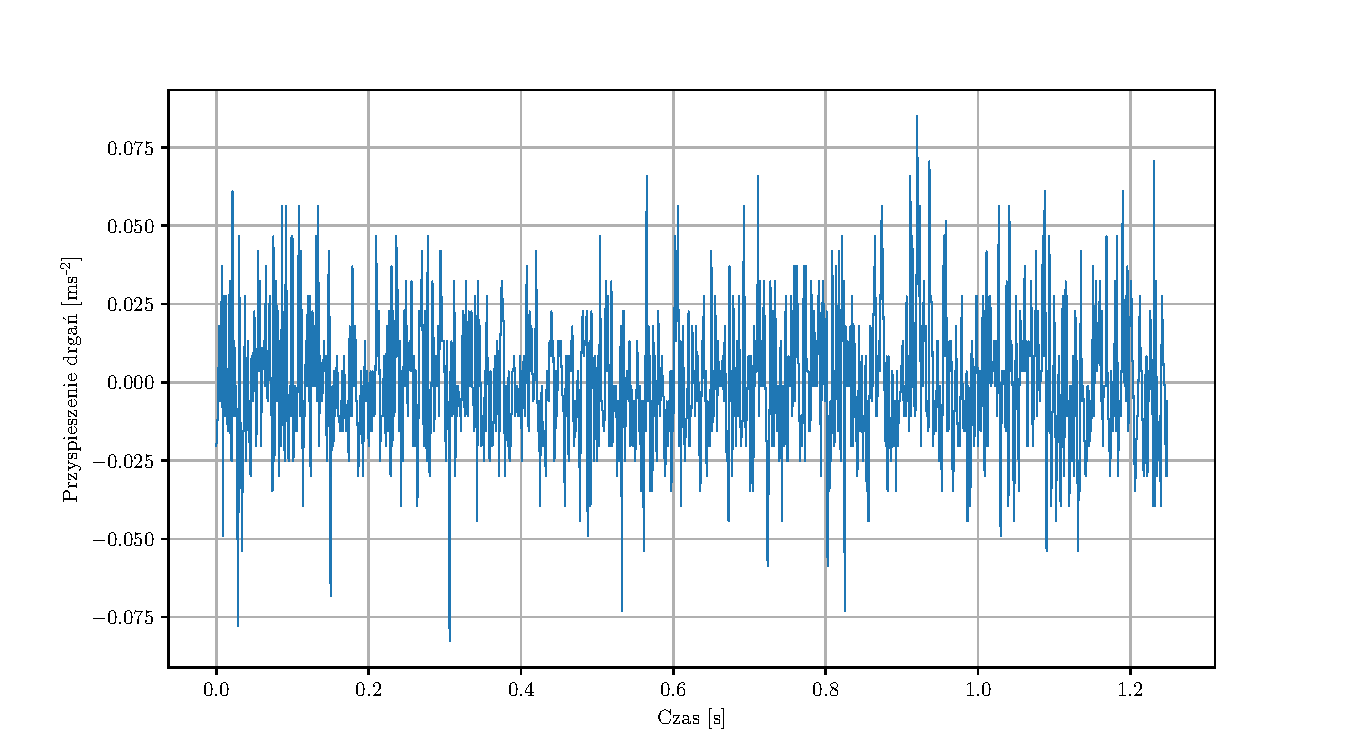
\includegraphics[width=\textwidth]{plots/accel_x.pdf}
  \caption{Fragment wibrogramu przyspieszenia drgań w osi X}
  \label{plot:accel_x}
\end{figure}

\begin{figure}[!tbh]
  \centering
  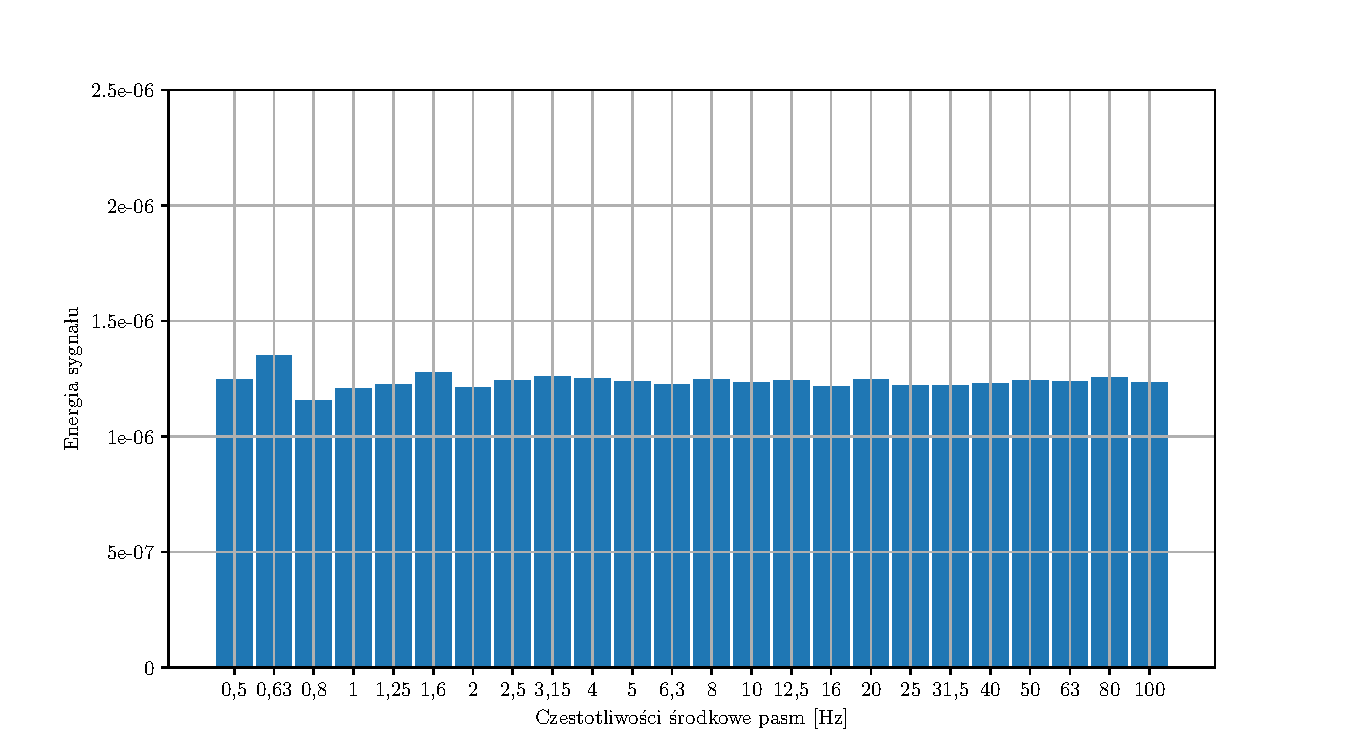
\includegraphics[width=\textwidth]{plots/power_x.pdf}
  \caption{Widmo energetyczne sygnału przyspieszenia drgań w osi X}
  \label{plot:power_x}
\end{figure}

\section{Wnioski}

% wnioski ogólne i dotyczące wyników

Należy pamiętać, że projekt ten jest częścią większego, mającego objąć swoim
zakresem pomiary zarówno drgań jak i hałasu środowiskowego. Stacje pomiarowe
wyposażone w akcelerometry oraz mikrofony rejestrowałyby dane, a następnie
wysyłały je na serwer sieciowy, gdzie byłyby one analizowane oraz przechowywane.
Dostęp do nich byłby możliwy przez aplikację hosta, gdzie można by było
przeglądać dane aktualne oraz analizować dane archiwalne.

\printbibliography[title=Bibliografia]

\end{document}
